\section{Performance analysis}

In this section we present the performance analysis and comparison of PeerDB-enabled queries vs. traditional approaches using relational DBMS and NoSQL database.

\subsection{Setup}

We approached the performance analysis by designing a simple data schema which consist of a one-to-many relation, many-to-many relation, and a reverse relation.
To easier understand it and discuss it, we assign to entities in the schema meaningful names of a simple blog application.
Figure \ref{schema} shows the entities and relations between them.

\begin{figure}[!h]
\centering
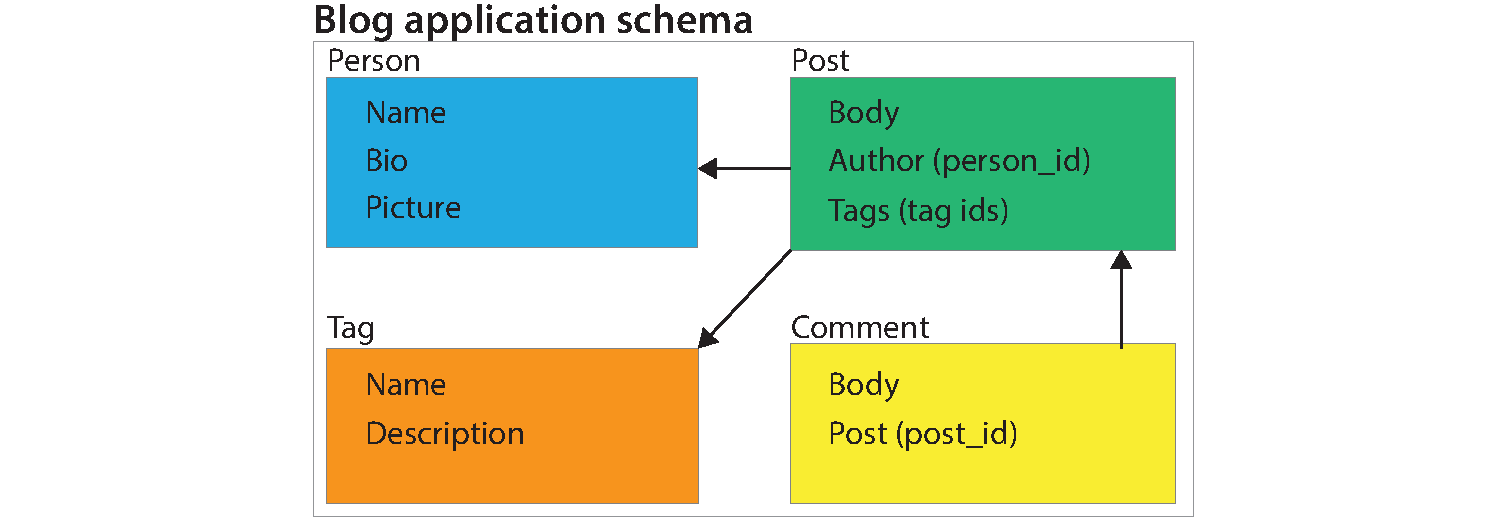
\includegraphics[width=0.9\columnwidth]{schema}
\caption{A blog post is the main entity we are querying. It has one-to-many \emph{author} relation to person entity and many-to-many \emph{tags} relation to tag entity. Comment entity has a one-to-many \emph{post} relation to the post entity, for which this relation is a reverse relation where we are interested in all comments made for a given post.}
\label{schema}
\end{figure}

To measure performance we decided to use a query which uses all relatons in the schema.
By querying for a blog post document, in addition to the post data itself, we want to get:
\begin{itemize}
\item name and picture of the author
\item name and description of all tags of the blog post
\item body of all blog post's comments
\end{itemize}

The concrete query we used is as follows: based on a string tag name, obtain all blog posts which are tagged with that tag, and for each blog post above mentioned additional data have to be available.

To be able to compare the measurements we implemented this schema and query in multiple systems:
\begin{itemize}
\item using PostgreSQL relational DBMS with low-level queries in Python
\item using PostgreSQL relational DBMS with high-level queries in Django, a Python based web framework
\item using MongoDB with low-level queries in Python
\item using MongoDB with high-level queries in Meteor
\item using MongoDB with PeerDB in Meteor
\item using MongoDB with PeerDB in Python
\end{itemize}

The motivation was to measure both low-level and high-level database interfaces to be able to compare difference between using a high-level web framework and not. To measure both traditional relational DBMS and NoSQL one. And of course to see how it works when using PeerDB and when not.

\begin{table}
  \small
  \begin{center}
  \begin{tabular}{|l|l|l|l|}
    %\hline
    \hline
    Entity & Number of documents\\
    \hline
    Person & 100 \\
    Tags & 100 \\ 
    Posts & 1000 \\ 
    Comments & 10000 \\ 
    \hline

  \end{tabular}
  \end{center}
  \caption{Basic number of documents used in the benchmark.}
  \label{numbers}
\end{table}

\begin{table}
  \small
  \begin{center}
  \begin{tabular}{|l|l|l|l|}
    %\hline
    \hline
    Field & Size in bytes\\
    \hline
    Person name & 11 \\
    Person bio & 1000 \\ 
    \emph{Person picture} & 10 \\
    Tag name & 11 \\ 
    \emph{Tag description} & 10 \\
    Post body & 1000 \\
    \emph{Comment body} & 10 \\
    \hline

  \end{tabular}
  \end{center}
  \caption{Basic size of fields in documents used in the benchmark.
  \emph{Emphasized} are fields which we varied in size.}
  \label{sizes}
\end{table}

Basic number of documents used in the benchmark are shown in table \ref{numbers}, and basic size of fields in documents used in the benchmark in table \ref{sizes}.
Basic number of tags per post was 10.
We uniformly distributed all comments across all blog posts. For future work we could consider using a long-tailed distribution.

We scaled this basic numbers and sizes to vary:
\begin{itemize}
\item number of documents, we used multiplication factors 1, 2, 4, 6, 8, 10
\item size of person picture, tag description, and comment body fields in documents, we used sizes 10, 100, 1000, 10000, 100000
\end{itemize}

When varying one dimension we kept the other at its basic value.

In addition, for two PeerDB based systems (Meteor and Python) we additionally vary how many PeerDB instances are observing and handling the changes in the database, running all above variations on 1, 2, 4, 6, 8 and 10 instances.

\subsection{Execution}

For execution of the benchmark we prepared a Docker image with Ubuntu 14.04.1 Linux as the base system, and PostgreSQL 9.3.5 and MongoDB 2.4.9.
We run that image on three Linux based 64bit systems, each with 32 GB of memory and 2 Intel Xeon X5670 2.93GHz processors with 6 cores each processor.
We varied the type of a running program and parameters when running an image to obtain the following measurements.

\subsection{Results}

\begin{figure}%
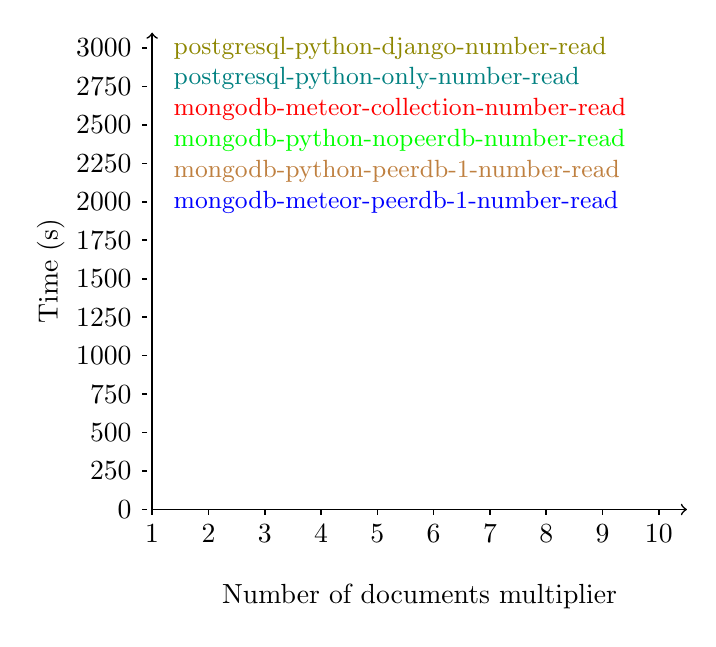
\begin{tikzpicture}[
	y=.003cm,
	x=1.1cm,
	semithick,
	scale=0.65
]

\draw[color=olive,thick] node[anchor=west] at (1.2,3000) {\small postgresql-python-django-number-read};
\draw[color=teal,thick] node[anchor=west] at (1.2,2800) {\small postgresql-python-only-number-read};
\draw[color=red,thick] node[anchor=west] at (1.2,2600) {\small mongodb-meteor-collection-number-read};
\draw[color=green,thick] node[anchor=west] at (1.2,2400) {\small mongodb-python-nopeerdb-number-read};
\draw[color=brown,thick] node[anchor=west] at (1.2,2200) {\small mongodb-python-peerdb-1-number-read};
\draw[color=blue,thick] node[anchor=west] at (1.2,2000) {\small mongodb-meteor-peerdb-1-number-read};

\draw[->] (1,0) -- coordinate (x axis) (10.5,0);
\draw[->] (1,0) -- coordinate (y axis) (1,3100);
\foreach \x in {1,...,10}
	\draw (\x,0pt) -- (\x,-3pt) node[anchor=north] {$\x$};
\foreach \y in {0,250,...,3000}
	\draw[xshift=1cm] (0pt,\y) -- (-3pt,\y) node[anchor=east] {$\y$};
\node[below=1.2cm,anchor=base] at (x axis) {Number of documents multiplier};
\node[left=1.2cm,rotate=90,anchor=base] at (y axis) {Time (s)};

\draw[color=red,thick] plot[mark=x,smooth] file {mongodb-meteor-collection-number-read.txt};
\draw[color=blue,thick] plot[mark=x,smooth] file {mongodb-meteor-peerdb-1-number-read.txt};
\draw[color=green,thick] plot[mark=x,smooth] file {mongodb-python-nopeerdb-number-read.txt};
\draw[color=brown,thick] plot[mark=x,smooth] file {mongodb-python-peerdb-1-number-read.txt};
\draw[color=olive,thick] plot[mark=x,smooth] file {postgresql-python-django-number-read.txt};
\draw[color=teal,thick] plot[mark=x,smooth] file {postgresql-python-only-number-read.txt};

\end{tikzpicture}%
\caption{number-read}%
\label{number-read}%
\end{figure}

\begin{figure}%
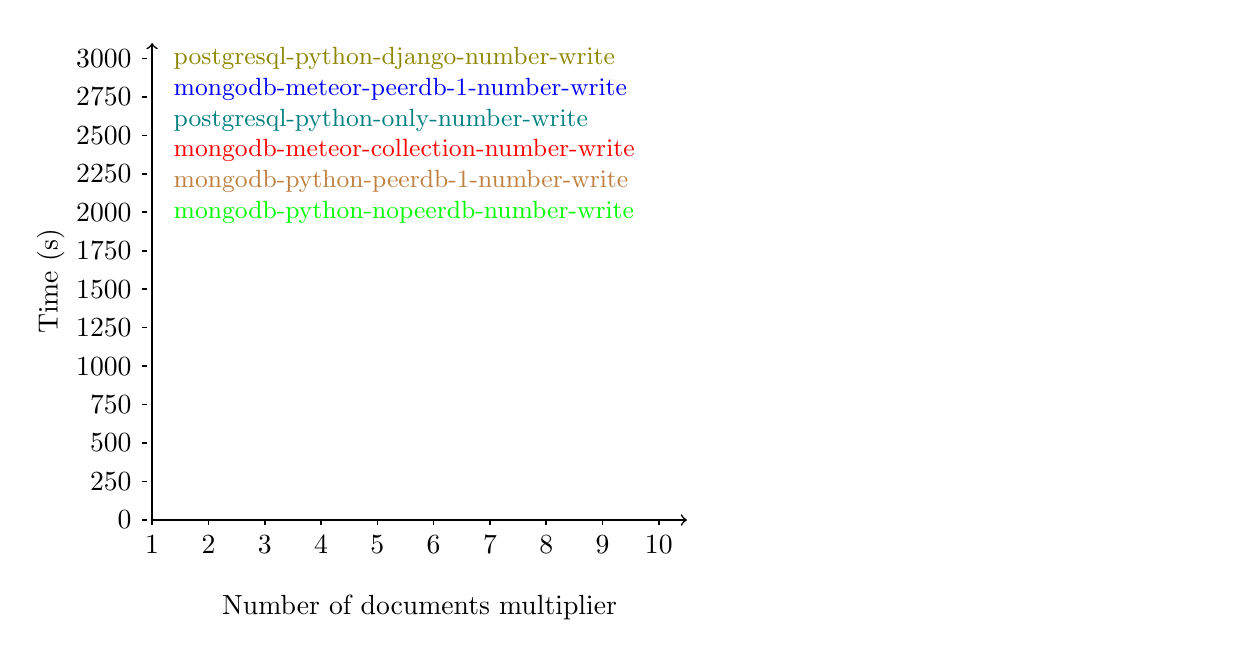
\begin{tikzpicture}[
	y=.003cm,
	x=1.1cm,
	semithick,
	scale=0.65
]

\draw[color=olive,thick] node[anchor=west] at (1.2,3000) {\small postgresql-python-django-number-write};
\draw[color=blue,thick] node[anchor=west] at (1.2,2800) {\small mongodb-meteor-peerdb-1-number-write};
\draw[color=teal,thick] node[anchor=west] at (1.2,2600) {\small postgresql-python-only-number-write};
\draw[color=red,thick] node[anchor=west] at (1.2,2400) {\small mongodb-meteor-collection-number-write};
\draw[color=brown,thick] node[anchor=west] at (1.2,2200) {\small mongodb-python-peerdb-1-number-write};
\draw[color=green,thick] node[anchor=west] at (1.2,2000) {\small mongodb-python-nopeerdb-number-write};

\draw[->] (1,0) -- coordinate (x axis) (10.5,0);
\draw[->] (1,0) -- coordinate (y axis) (1,3100);
\foreach \x in {1,...,10}
	\draw (\x,0pt) -- (\x,-3pt) node[anchor=north] {$\x$};
\foreach \y in {0,250,...,3000}
	\draw[xshift=1cm] (0pt,\y) -- (-3pt,\y) node[anchor=east] {$\y$};
\node[below=1.2cm,anchor=base] at (x axis) {Number of documents multiplier};
\node[left=1.2cm,rotate=90,anchor=base] at (y axis) {Time (s)};

\clip (-1,-100) rectangle (20,3200);

\draw[color=red,thick] plot[mark=x,smooth] file {mongodb-meteor-collection-number-write.txt};
\draw[color=blue,thick] plot[mark=x,smooth] file {mongodb-meteor-peerdb-1-number-write.txt};
\draw[color=green,thick] plot[mark=x,smooth] file {mongodb-python-nopeerdb-number-write.txt};
\draw[color=brown,thick] plot[mark=x,smooth] file {mongodb-python-peerdb-1-number-write.txt};
\draw[color=olive,thick] plot[mark=x,smooth] file {postgresql-python-django-number-write.txt};
\draw[color=teal,thick] plot[mark=x,smooth] file {postgresql-python-only-number-write.txt};

\end{tikzpicture}%
\caption{number-write}%
\label{number-write}%
\end{figure}

\begin{figure}%
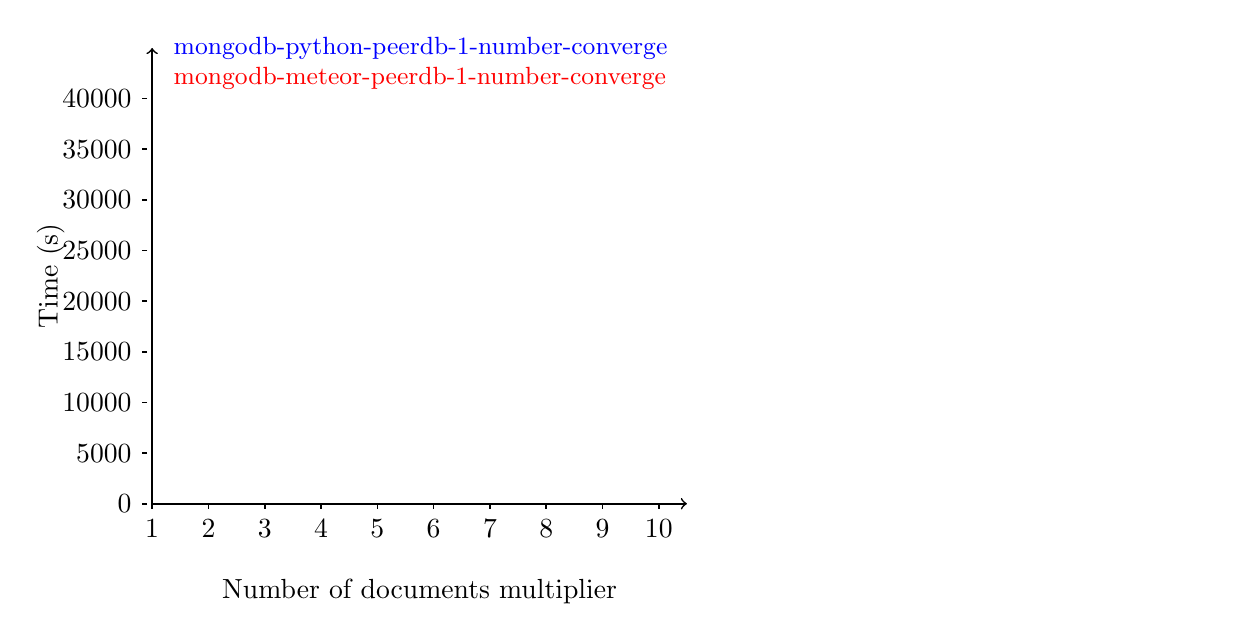
\begin{tikzpicture}[
	y=.0002cm,
	x=1.1cm,
	semithick,
	scale=0.65
]

\draw[color=blue,thick] node[anchor=west] at (1.2,45000) {\small mongodb-python-peerdb-1-number-converge};
\draw[color=red,thick] node[anchor=west] at (1.2,42000) {\small mongodb-meteor-peerdb-1-number-converge};

\draw[->] (1,0) -- coordinate (x axis) (10.5,0);
\draw[->] (1,0) -- coordinate (y axis) (1,45000);
\foreach \x in {1,...,10}
	\draw (\x,0pt) -- (\x,-3pt) node[anchor=north] {$\x$};
\draw[xshift=1cm] (0pt,0) -- (-3pt,0) node[anchor=east] {$0$};
\draw[xshift=1cm] (0pt,5000) -- (-3pt,5000) node[anchor=east] {$5000$};
\draw[xshift=1cm] (0pt,10000) -- (-3pt,10000) node[anchor=east] {$10000$};
\draw[xshift=1cm] (0pt,15000) -- (-3pt,15000) node[anchor=east] {$15000$};
\draw[xshift=1cm] (0pt,20000) -- (-3pt,20000) node[anchor=east] {$20000$};
\draw[xshift=1cm] (0pt,25000) -- (-3pt,25000) node[anchor=east] {$25000$};
\draw[xshift=1cm] (0pt,30000) -- (-3pt,30000) node[anchor=east] {$30000$};
\draw[xshift=1cm] (0pt,35000) -- (-3pt,35000) node[anchor=east] {$35000$};
\draw[xshift=1cm] (0pt,40000) -- (-3pt,40000) node[anchor=east] {$40000$};
\node[below=1.2cm,anchor=base] at (x axis) {Number of documents multiplier};
\node[left=1.2cm,rotate=90,anchor=base] at (y axis) {Time (s)};

\clip (-1,-100) rectangle (20,46000);

\draw[color=red,thick] plot[mark=x,smooth] file {mongodb-meteor-peerdb-1-number-converge.txt};
\draw[color=blue,thick] plot[mark=x,smooth] file {mongodb-python-peerdb-1-number-converge.txt};

\end{tikzpicture}%
\caption{number-converge}%
\label{number-converge}%
\end{figure}

\begin{figure}%
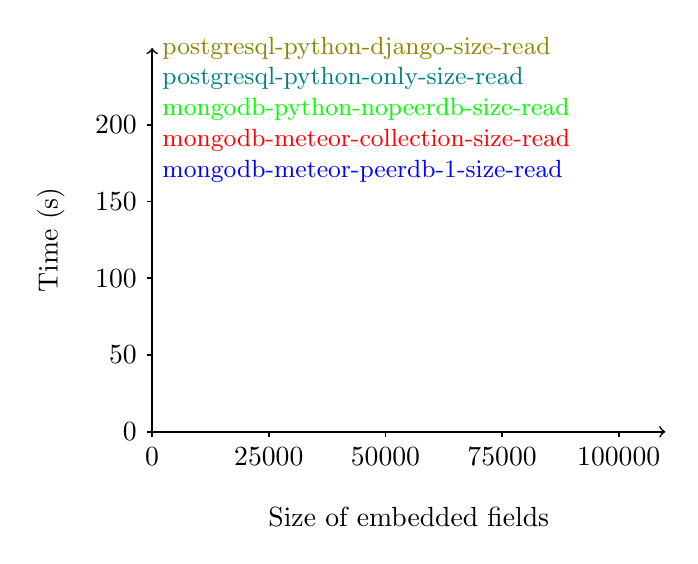
\begin{tikzpicture}[
	y=.03cm,
	x=0.00009cm,
	semithick,
	scale=0.65
]

\draw[color=olive,thick] node[anchor=west] at (1.2,250) {\small postgresql-python-django-size-read};
\draw[color=teal,thick] node[anchor=west] at (1.2,230) {\small postgresql-python-only-size-read};
\draw[color=green,thick] node[anchor=west] at (1.2,210) {\small mongodb-python-nopeerdb-size-read};
\draw[color=red,thick] node[anchor=west] at (1.2,190) {\small mongodb-meteor-collection-size-read};
\draw[color=blue,thick] node[anchor=west] at (1.2,170) {\small mongodb-meteor-peerdb-1-size-read};
%\draw[color=brown,thick] node[anchor=west] at (1.2,2200) {\small mongodb-python-peerdb-1-size-read};

\draw[->] (1,0) -- coordinate (x axis) (110000,0);
\draw[->] (1,0) -- coordinate (y axis) (1,250);
\foreach \x in {0,25000,50000,75000,100000}
	\draw (\x,0pt) -- (\x,-3pt) node[anchor=north] {$\x$};
\foreach \y in {0,50,...,200}
	\draw[xshift=0cm] (0pt,\y) -- (-3pt,\y) node[anchor=east] {$\y$};
\node[below=1.2cm,anchor=base] at (x axis) {Size of embedded fields};
\node[left=1.2cm,rotate=90,anchor=base] at (y axis) {Time (s)};

\draw[color=red,thick] plot[mark=x,smooth] file {mongodb-meteor-collection-size-read.txt};
\draw[color=blue,thick] plot[mark=x,smooth] file {mongodb-meteor-peerdb-1-size-read.txt};
\draw[color=green,thick] plot[mark=x,smooth] file {mongodb-python-nopeerdb-size-read.txt};
%\draw[color=brown,thick] plot[mark=x,smooth] file {mongodb-python-peerdb-1-size-read.txt};
\draw[color=olive,thick] plot[mark=x,smooth] file {postgresql-python-django-size-read.txt};
\draw[color=teal,thick] plot[mark=x,smooth] file {postgresql-python-only-size-read.txt};

\end{tikzpicture}%
\caption{size-read}%
\label{size-read}%
\end{figure}

\begin{figure}%
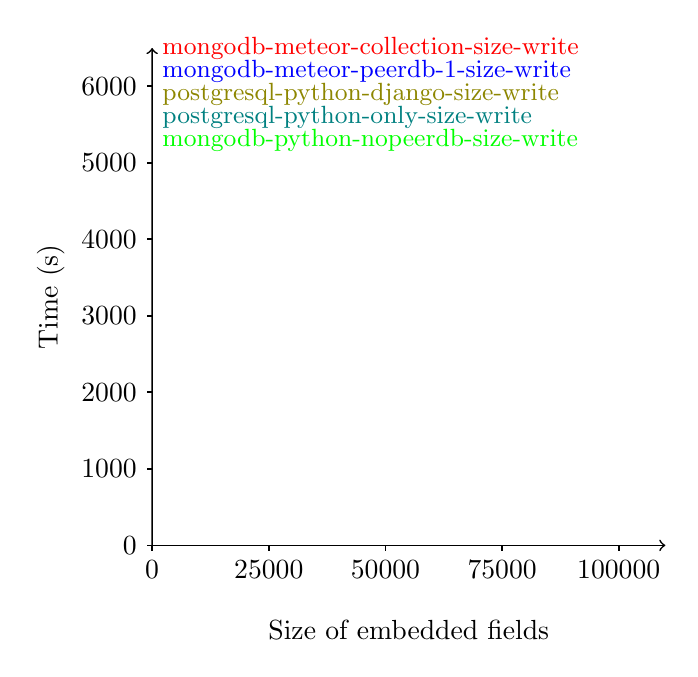
\begin{tikzpicture}[
	y=.0015cm,
	x=0.00009cm,
	semithick,
	scale=0.65
]

\draw[color=red,thick] node[anchor=west] at (1.2,6500) {\small mongodb-meteor-collection-size-write};
\draw[color=blue,thick] node[anchor=west] at (1.2,6200) {\small mongodb-meteor-peerdb-1-size-write};
\draw[color=olive,thick] node[anchor=west] at (1.2,5900) {\small postgresql-python-django-size-write};
\draw[color=teal,thick] node[anchor=west] at (1.2,5600) {\small postgresql-python-only-size-write};
\draw[color=green,thick] node[anchor=west] at (1.2,5300) {\small mongodb-python-nopeerdb-size-write};
%\draw[color=brown,thick] node[anchor=west] at (1.2,2200) {\small mongodb-python-peerdb-1-size-write};

\draw[->] (1,0) -- coordinate (x axis) (110000,0);
\draw[->] (1,0) -- coordinate (y axis) (0,6500);
\foreach \x in {0,25000,50000,75000,100000}
	\draw (\x,0pt) -- (\x,-3pt) node[anchor=north] {$\x$};
\foreach \y in {0,1000,...,6500}
	\draw[xshift=0cm] (0pt,\y) -- (-3pt,\y) node[anchor=east] {$\y$};
\node[below=1.2cm,anchor=base] at (x axis) {Size of embedded fields};
\node[left=1.2cm,rotate=90,anchor=base] at (y axis) {Time (s)};

\draw[color=red,thick] plot[mark=x,smooth] file {mongodb-meteor-collection-size-write.txt};
\draw[color=blue,thick] plot[mark=x,smooth] file {mongodb-meteor-peerdb-1-size-write.txt};
\draw[color=green,thick] plot[mark=x,smooth] file {mongodb-python-nopeerdb-size-write.txt};
%\draw[color=brown,thick] plot[mark=x,smooth] file {mongodb-python-peerdb-1-size-write.txt};
\draw[color=olive,thick] plot[mark=x,smooth] file {postgresql-python-django-size-write.txt};
\draw[color=teal,thick] plot[mark=x,smooth] file {postgresql-python-only-size-write.txt};

\end{tikzpicture}%
\caption{size-write}%
\label{size-write}%
\end{figure}

\begin{figure}%
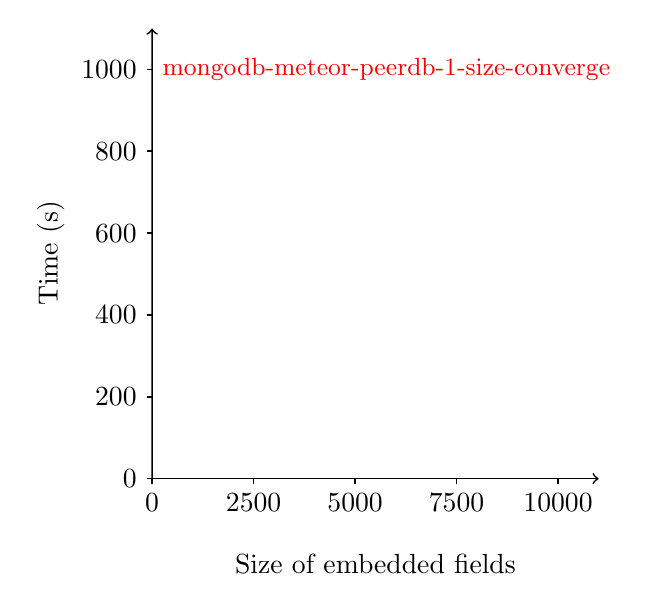
\begin{tikzpicture}[
	y=.008cm,
	x=.0008cm,
	semithick,
	scale=0.65
]

\draw[color=red,thick] node[anchor=west] at (1.2,1000) {\small mongodb-meteor-peerdb-1-size-converge};
%\draw[color=blue,thick] node[anchor=west] at (1.2,900) {\small mongodb-python-peerdb-1-size-converge};

\draw[->] (1,0) -- coordinate (x axis) (11000,0);
\draw[->] (1,0) -- coordinate (y axis) (0,1100);
\foreach \x in {0,2500,...,11000}
	\draw (\x,0pt) -- (\x,-3pt) node[anchor=north] {$\x$};
\foreach \y in {0,200,...,1000}
	\draw[xshift=0cm] (0pt,\y) -- (-3pt,\y) node[anchor=east] {$\y$};
\node[below=1.2cm,anchor=base] at (x axis) {Size of embedded fields};
\node[left=1.2cm,rotate=90,anchor=base] at (y axis) {Time (s)};

\draw[color=red,thick] plot[mark=x,smooth] file {mongodb-meteor-peerdb-1-size-converge.txt};
%\draw[color=blue,thick] plot[mark=x,smooth] file {mongodb-python-peerdb-1-size-converge.txt};

\end{tikzpicture}%
\caption{size-converge}%
\label{size-converge}%
\end{figure}

